\section{Dreiphasiger Wechselrichter}

\subsection{Grundschaltung}

% --- bestehende Grafik: Dreiphasen-Brücke ---
\begin{center}
    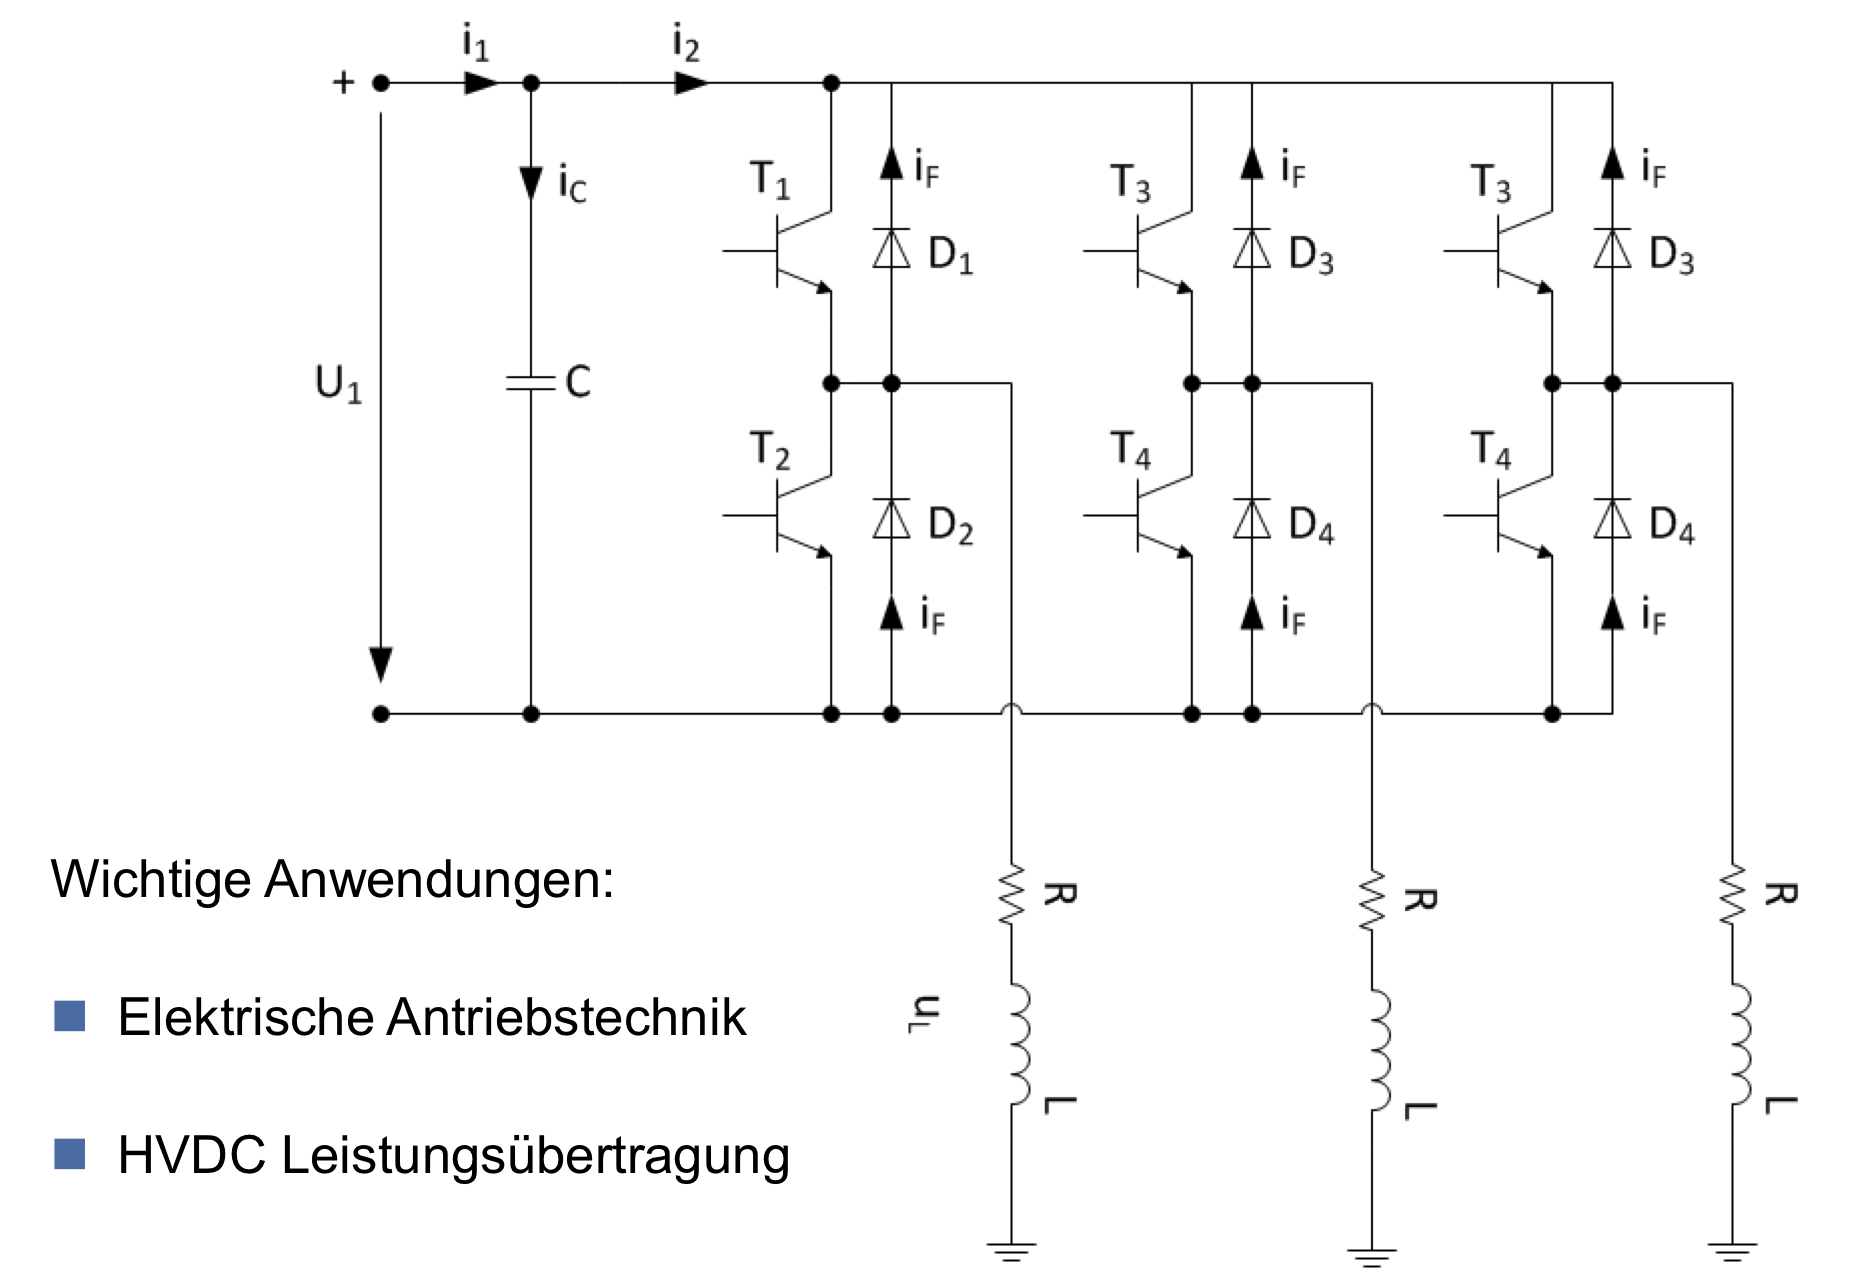
\includegraphics[width=0.85\linewidth]{images/3PWechselrichter.png}
\end{center}
Der dreiphasige Wechselrichter erzeugt aus $U_{DC}$ drei um $120^\circ$ phasenverschobene Spannungen.

\subsection{180$^\circ$-Betrieb}

% --- bestehende Grafik: 180 Grad Betrieb ---

Eigenschaften:
\begin{itemize}
    \item Jedes Ventil leitet 180$^\circ$
    \item Gute Ausnutzung der Gleichspannung
\end{itemize}

\subsection{120$^\circ$-Betrieb}


Eigenschaften:
\begin{itemize}
    \item Jedes Ventil leitet 120$^\circ$
    \item Geringere Schaltverluste
\end{itemize}

\subsection{Leiterspannungen und Grundschwingung}

Leiterspannung:
\[
\cbl{u_{LL} = u_a - u_b}
\]

Grundschwingungsamplitude:
\[
\cbl{\hat U_{LL,1} = \sqrt{3} \, \hat U_{ph,1}}
\]

\subsection{Vergleich Einphasig -- Dreiphasig}

\begin{center}
\begin{tabular}{l|c|c}
 & Einphasig & Dreiphasig \\ \hline
Phasen & 1 & \cbl{3} \\
Leistungsfluss & pulsierend & \cbl{konstant} \\
Oberschwingungen & hoch & \cbl{geringer} \\
\end{tabular}
\end{center}

\subsection{Merksätze}

\begin{itemize}
    \item PWM bestimmt Amplitude und Frequenz.
    \item 180$^\circ$- und 120$^\circ$-Betrieb unterscheiden sich in Leitintervallen.
    \item Dreiphasige Systeme liefern konstanten Leistungsfluss.
\end{itemize}
